\section{Results}
\label{sec:result}

The results first record how often paths enter the feasible inter-region
candidate space, then compare network and corridor concentration within the
same candidate-bearing observations. Layer Agreement is the primary cross-
layer summary. Absolute exposure and breadth remain separate results because
they use different denominators and answer different questions.

The processing pipeline retains 490,911 valid traceroutes from 707,314 raw
records and yields 3,291,063 atomic segments. Of 2,432,559 mappable segments,
555,119 reach candidate landing points, 171,232 satisfy the corridor
constraints, and 124,350 support at least one feasible inter-region corridor.
The equal-share audit records 71,990 single-corridor and 52,360 bounded multi-
corridor segments. After the eligibility filters in Section
~\ref{sec:framework_path_segmentation}, the analysis contains 370 auditable
country--measurement units: 222 DNS Root, 53 application, and 95 topology-
reference units.

\subsection{Inter-Region Candidate Exposure}
\label{subsec:overall-exposure}

Inter-region candidates occur infrequently for most service-facing
populations. The DNS family contains 945 country--measurement units with at
least 30 valid traceroutes across 77 countries. Pooling eligible Root
observations within each country by valid-trace count yields median DNS
exposure of 5.50\% (IQR 1.10--23.04\%; mean 17.80\%). The difference between
the median and mean records a pronounced upper tail across countries.

The three application measurements occupy the same low-exposure range. Median
country--measurement exposure is 1.90\% for Wikipedia, 1.96\% for Reddit, and
1.43\% for Netflix Assets. The dynamic multi-target topology references reach
23.24\% for MSM~5051 and 23.81\% for MSM~5151. These figures describe how
often paths in each observed population contain a feasible inter-region
corridor; they do not describe concentration after entry.

Country-matched comparisons retain source geography while changing the target
population. DNS exposure is lower than MSM~5051 in 70 of 77 shared countries,
with a median paired difference of -14.52 percentage points. It is lower than
MSM~5151 in 54 of 59 shared countries, with a median difference of -14.82
points. The paired direction holds for 90.9\% and 91.5\% of shared countries,
respectively. Because the target populations differ by design, the comparison
is descriptive and does not identify a deployment or target-selection effect.

\begin{figure*}[t]
  \centering
  \subfloat[Country--measurement exposure.\label{fig:result-overview-distribution}]{%
    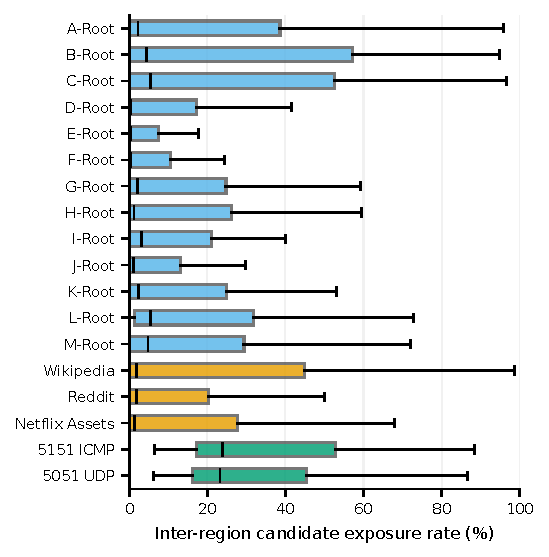
\includegraphics[width=0.39\textwidth]{figures/fig_result_overview_distribution.pdf}}
  \hspace{0.045\textwidth}
  \subfloat[Country-matched comparison.\label{fig:result-overview-paired}]{%
    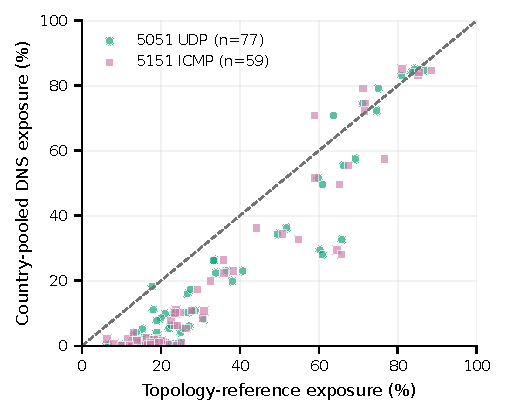
\includegraphics[width=0.34\textwidth]{figures/fig_result_overview_paired.pdf}}
  \caption{Inter-region candidate exposure in the observed measurement
  populations.}
  \label{fig:result-overview}
\end{figure*}

\subsection{Layer Agreement Differs by Geography}
\label{subsec:geographic-agreement}

The association between network and corridor concentration differs across the
observed service-facing geographic groups. Under projection-score weighting,
Layer Agreement is 0.632 across 67 island and archipelagic units and 0.001
across 202 coastal-mainland units. The observed coefficient difference is
0.631. Landlocked units are not included in either group. No clustered
uncertainty interval is available in the existing experiment set, so the
coefficients are reported as descriptive associations without a significance
claim.

\begin{table}[t]
  \centering
  \caption{Service-facing Layer Agreement by geography and allocation rule.}
  \label{tab:geographic-agreement}
  \footnotesize
  \setlength{\tabcolsep}{3.3pt}
  \begin{tabular}{lrrr}
    \toprule
    Allocation & Island/arch. & Coastal mainland & Difference \\
    \midrule
    Equal share & 0.380 & -0.081 & 0.461 \\
    Projection score & 0.632 & 0.001 & 0.631 \\
    Top-1 & 0.820 & 0.105 & 0.715 \\
    \bottomrule
  \end{tabular}
\end{table}

The geographic contrast remains in the same direction under all three
candidate-allocation rules. As allocation moves from equal shares to
projection-score weighting and then Top-1, the island coefficient increases
from 0.380 to 0.632 and 0.820, while the coastal-mainland coefficient changes
from -0.081 to 0.001 and 0.105. The between-group difference consequently
increases from 0.461 to 0.631 and 0.715. This monotonic change shows that the
measured association is sensitive to how ambiguous corridor mass is allocated,
but the geographic ordering does not depend on one allocation rule. Without
physical-route ground truth, the comparison does not establish that one rule
recovers the true association.

The result does not imply that geography causes the two layers to agree or
disagree. It records how the two concentration rankings relate within the
measured snapshot. A mechanism that would explain the difference requires
additional evidence beyond these coefficients.

\subsection{Absolute Exposure and Breadth by Geography}
\label{subsec:geography}

The geographic groups also differ in how often DNS paths enter the candidate
space. Giving each country equal weight, island and archipelagic countries have
median country-pooled DNS exposure of 49.61\% across 9 countries, compared
with 7.88\% for 54 other coastal countries and 1.70\% for 14 landlocked
countries. This ordering concerns exposure, not Layer Agreement.

Conditional equal-share corridor breadth follows a different ordering. Island
and archipelagic countries have median corridor Top-2 share of 53.3\% and 5.58
effective corridors. Other coastal countries reach 75.4\% and 3.39. The two
represented landlocked countries reach 80.2\% and 2.51. Across 38 countries
with both pooled exposure and an auditable corridor summary, exposure has
Spearman association -0.29 with corridor Top-2 share and 0.30 with effective
corridor count. These quantities show that frequent entry and conditional
concentration are not interchangeable.

\begin{figure*}[t]
  \centering
  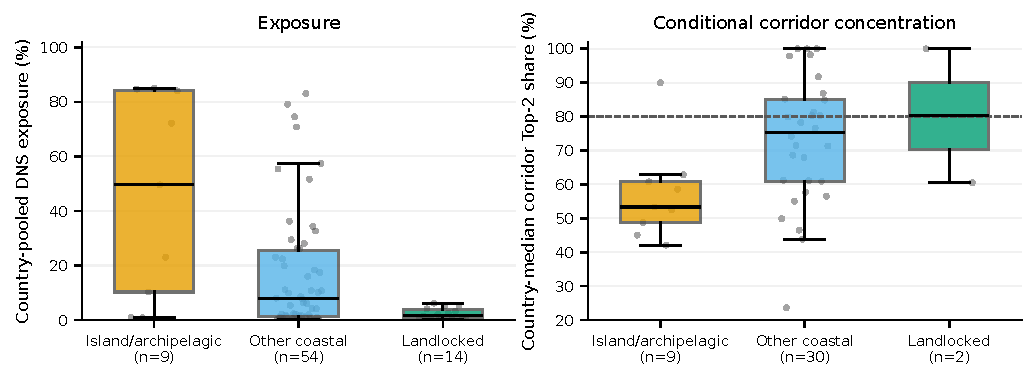
\includegraphics[width=0.72\textwidth]{figures/fig_country_geography_30km.pdf}
  \caption{DNS exposure and equal-share corridor concentration by geography.
  Country counts refer to the DNS country-level summary and are distinct from
  the service-facing unit counts in Table~\ref{tab:geographic-agreement}.}
  \label{fig:country-geography}
\end{figure*}

\subsection{Layer Agreement within Measurement Families}
\label{subsec:family-agreement}

Family-level coefficients do not reproduce the geographic separation. Table
~\ref{tab:family-agreement} reports Layer Agreement within each observed
measurement family. Under projection-score weighting, the coefficient is
0.176 for 219 DNS units, 0.229 for 53 application units, and 0.012 for 95
topology-reference units. Equal-share and Top-1 allocation change all three
coefficients, with the largest change occurring for DNS Roots. The existing
artifacts contain 222 DNS units in the equal-share audit and 219 in the family
allocation comparison; the status of the remaining three must be reconciled
before a final artifact release.

\begin{table}[t]
  \centering
  \caption{Layer Agreement by measurement family.}
  \label{tab:family-agreement}
  \footnotesize
  \setlength{\tabcolsep}{4.0pt}
  \begin{tabular}{lrrrr}
    \toprule
    Family & \(n\) & Equal & Score & Top-1 \\
    \midrule
    DNS Roots & 219 & 0.096 & 0.176 & 0.330 \\
    Applications & 53 & 0.030 & 0.229 & 0.372 \\
    Topology references & 95 & 0.139 & 0.012 & 0.122 \\
    \bottomrule
  \end{tabular}
\end{table}

Absolute equal-share corridor breadth also differs among the observed
families. Table~\ref{tab:family-summary} reports network and corridor medians.
DNS Roots and applications have median corridor Top-2 shares of 72.0\% and
70.3\%, compared with 30.6\% for topology references. Their median effective
corridor counts are 3.84 and 3.51, compared with 18.01. These are summaries of
different target populations, not a controlled estimate of a service effect.

\begin{table*}[t]
  \centering
  \caption{Equal-share network-transition and corridor distributions.}
  \label{tab:family-summary}
  \footnotesize
  \setlength{\tabcolsep}{4.0pt}
  \begin{tabular}{lrrrrrr}
    \toprule
    Family & Units & Net. Top-2 & Corr. Top-2 & \(\Delta\)Top-2
      & Eff. network & Eff. corridor \\
    \midrule
    DNS Roots & 222 & 53.1\% & 72.0\% & +11.0 pp & 7.45 & 3.84 \\
    Applications & 53 & 45.2\% & 70.3\% & +21.0 pp & 9.89 & 3.51 \\
    Topology references & 95 & 27.3\% & 30.6\% & +2.7 pp & 24.34 & 18.01 \\
    \bottomrule
  \end{tabular}
\end{table*}

The high-concentration tail follows the same descriptive family ordering. The
leading two corridors receive at least 80\% of mass in 83 of 222 DNS units
(37.4\%), 16 of 53 application units (30.2\%), and 4 of 95 topology-reference
units (4.2\%). Wikipedia, Reddit, and Netflix Assets have median corridor
Top-2 shares of 68.3\%, 71.0\%, and 71.6\%, with 4.25, 3.25, and 3.47 effective
corridors. Their median Top-2 shifts are 11.0, 25.6, and 23.6 percentage
points, respectively.

\begin{figure*}[t]
  \centering
  \subfloat[Corridor Top-2 share.\label{fig:corridor-top2-ecdf}]{%
    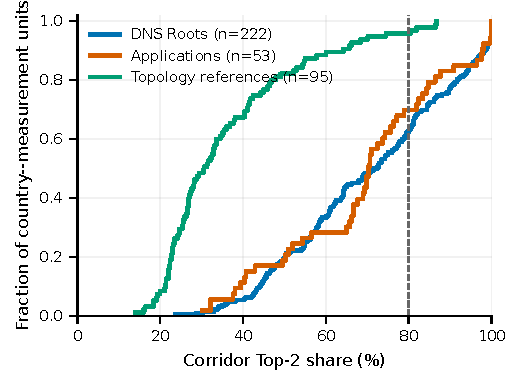
\includegraphics[width=0.36\textwidth]{figures/fig_corridor_concentration_ecdf.pdf}}
  \hspace{0.05\textwidth}
  \subfloat[Effective category counts.\label{fig:effective-counts}]{%
    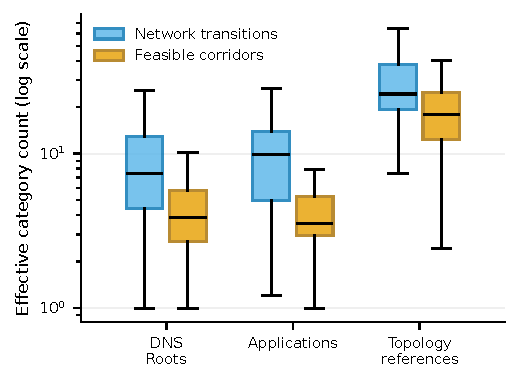
\includegraphics[width=0.36\textwidth]{figures/fig_effective_count_comparison.pdf}}
  \caption{Equal-share corridor concentration and breadth by measurement
  family. The families contain different target populations.}
  \label{fig:corridor-breadth}
\end{figure*}

Normalized entropy supplies a support-relative view. Median entropy reduction
is 0.126 for DNS Roots, 0.164 for applications, and 0.081 for topology
references. The family summaries therefore agree on observed absolute breadth
and concentration, while the Layer Agreement coefficients show that within-
family rankings remain weak and allocation-sensitive.

\subsection{Cross-Layer Outcomes Are Heterogeneous}
\label{subsec:cross-layer}

The 80\% Top-2 threshold identifies several service-facing outcomes rather
than a universal contraction. Among 275 service-facing units, 81 (29.5\%) are
network-broad/corridor-concentrated, 158 (57.5\%) remain broad at both layers,
18 (6.5\%) are concentrated at both, and 18 (6.5\%) are network-concentrated/
corridor-broad. Four of 95 topology-reference units (4.2\%) enter the first
class; the other 91 remain broad at both layers.

DNS Roots and applications enter the network-broad/corridor-concentrated class
at similar rates: 66 of 222 DNS units (29.7\%) and 15 of 53 application units
(28.3\%). Their median continuous Top-2 shifts are 11.0 and 21.0 percentage
points. Across all service-facing units, corridor Top-2 share increases in 184
of 275 (66.9\%), and effective category count contracts in 204 (74.2\%). Of
239 units with a broad network distribution, 178 (74.5\%) move upward in Top-2
share: 81 cross the threshold, while 97 remain broad at both layers with a
median increase of 6.3 percentage points.

\begin{figure*}[t]
  \centering
  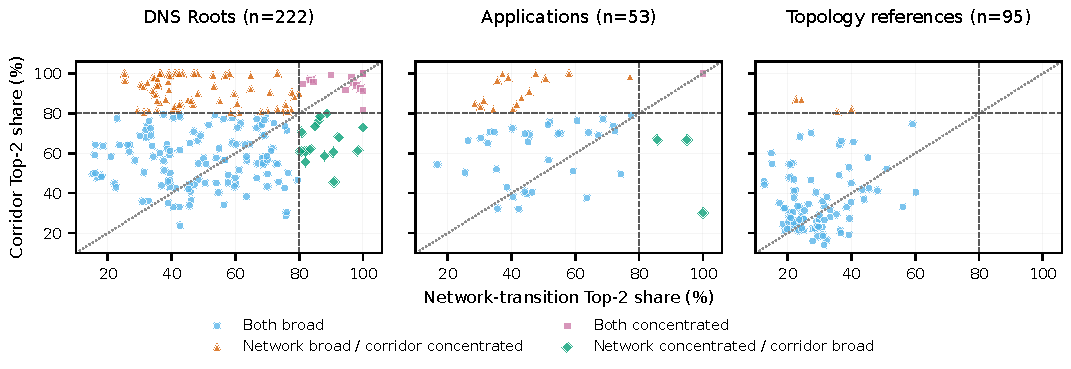
\includegraphics[width=0.92\textwidth]{figures/fig_cross_layer_distribution.pdf}
  \caption{Equal-share network-transition and corridor Top-2 shares for 370
auditable units. The 80\% lines define the descriptive four-class view; the
diagonal separates increases from decreases in concentration.}
  \label{fig:cross-layer}
\end{figure*}

Three existing cases distinguish continuous narrowing, expansion, and changes
in absolute breadth from support-relative evenness. \textbf{Singapore--
Netflix} moves from 32.5\% network Top-2 share to 65.0\% corridor Top-2 share,
while its effective count contracts from 19.86 to 3.41. It narrows without
crossing the 80\% threshold. \textbf{New Zealand--Netflix} moves from 63.6\%
to 37.6\%, with effective count expanding from 5.18 to 6.92.
\textbf{Singapore--H-Root} moves from 39.6\% to 50.1\%, and its effective
count contracts from 20.67 to 5.99 while normalized entropy changes only
slightly.

Bounded multi-corridor segments account for 99.9\%, 78.1\%, and 98.2\% of
candidate-bearing observations in these three cases. Repeated overlap among
the bounded sets produces different aggregate distributions under the same
projection and aggregation rules. The cases and four-class counts show why
neither a universal contraction claim nor a single retention ratio represents
the measured service-facing population.